% 泰勒展开
% 微积分|导数|高阶导数|泰勒展开|泰勒级数

\pentry{阶乘\upref{factor}, 高阶导数\upref{HigDer}, 分部积分法\upref{IntBP}}

若函数 $f$ 在开区间 $I$ 内可以求任意阶的导数(例如幂函数,三角函数,指数函数,对数函数等),那么这个函数可以用多项式近似,且在某种意义下, 总项数 $N$ 越多,近似得越精确. 确切地说, 对于任何$x_0\in I$, 存在唯一一个数列$\{c_n\}$, 使得对于任何正整数$N$, 皆有
\begin{equation}\label{Taylor_eq1}
f(x) -\sum_{n = 0}^N  c_n (x - x_0)^n=\order{|x-x_0|^{N+1}}.
\end{equation}
每一个系数$c_n$由函数在 $x_0$ 处的第 $n$ 阶导数求得
\begin{equation}\label{Taylor_eq2}
c_n = \frac{1}{n!} f^{(n)}(x_0);
\end{equation}
注意其中 0 的阶乘为 $0! = 1$. 另外由\autoref{Taylor_eq1} 得,当 $x=x_0$ 时,函数值等于多项式值. 当项数 $N$ 有限时,通常 $\abs{x-x_0}$ 越小多项式就越接近函数 . 以上这种把函数展开成多项式的方法就叫\textbf{泰勒展开(Taylor expansion)}, 得到的多项式叫做\textbf{泰勒级数(Taylor series)}. 我们先来看一个例子:

\begin{example}{正弦函数}
我们在 $x_0=0$ 处展开 $\sin x$, 由\autoref{Taylor_eq1} 和\autoref{Taylor_eq2} 得
\begin{equation}\label{Taylor_eq3}
\sin x = x - \frac{1}{3!}{x^3} + \frac{1}{5!}{x^5} - \frac{1}{7!} x^7 + \ldots 
\end{equation}
取不同的项数 $N$ 求和,画图如\autoref{Taylor_fig1}. 可见随着项数增加,多项式慢慢趋近正弦函数.

\begin{figure}[ht]
\centering
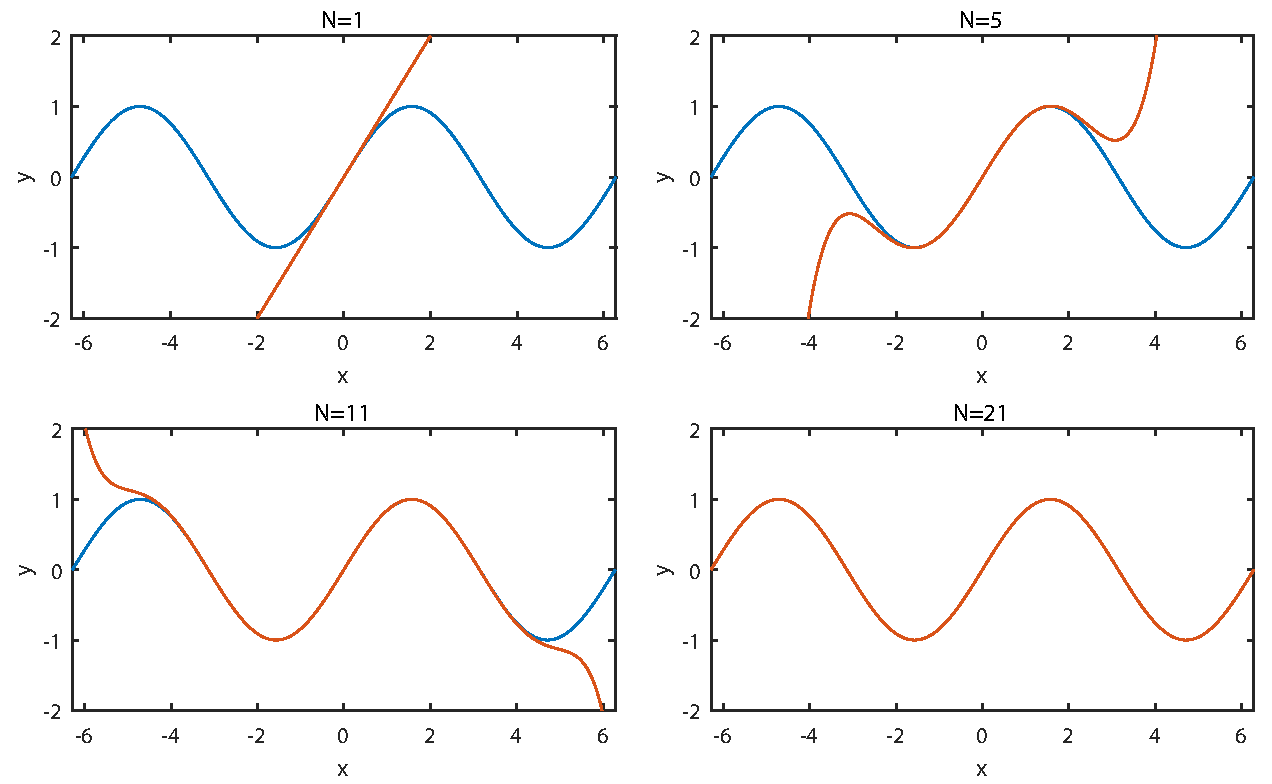
\includegraphics[width=14cm]{./figures/Taylor_1.pdf}
\caption{$\sin x$ 在原点处的泰勒展开的前 $N$ 项求和.容易看出,求和的项数越多,多项式(橙)与 $\sin x$ (蓝)吻合得越好.}\label{Taylor_fig1}
\end{figure}
\end{example}

\subsection{幼稚的推导}
这里给出一个比较直观的对比系数推导方法, 可能对初学者有一定启发或者帮助记忆. 但以后会看到这是不严谨的.

我们假设当项数 $N \to \infty$ 时, 存在唯一的多项式在某区间内处处趋于无穷可导函数 $f(x)$,即
\begin{equation}\label{Taylor_eq5}
f(x) = \sum_{n = 0}^\infty  c_n (x - x_0)^n
\end{equation}
首先代入 $x = x_0$,可得第一个系数 $c_0 = f(x_0)$. 现在我们对上式两边在 $x_0$ 处求导,得
\begin{equation}
f'(x_0) = c_1 + \eval{ \sum_{n = 2}^\infty n c_n (x - x_0)^{n - 1} }_{x = x_0}  = c_1
\end{equation}
如果对\autoref{Taylor_eq5} 两边在 $x_0$ 处求二阶导数,得
\begin{equation}
f''(x_0) = 2 c_2 + \eval{ \sum_{n = 3}^\infty  n(n - 1) c_n (x - x_0)^{n - 2} }_{x = x_0}  = 2 c_2
\end{equation}
即 $c_2 = f''(x_0)/2!$.  以此类推,如果对\autoref{Taylor_eq5} 两边在 $x_0$ 处求 $m$ 阶导数得
\begin{equation}
f^{(m)}(x_0) = m! c_m + \eval{ \sum_{n = m + 1}^\infty  \frac{n!}{(n - m)!} c_n (x - x_0)^{n - m} }_{x = x_0}  = m! c_m
\end{equation}
所以系数公式为
\begin{equation}
{c_m} = \frac{1}{m!} f^{(m)}(x_0)
\end{equation}

泰勒展开的存在说明了一些函数(下文的\textbf{解析函数})具有这样的性质:任何一点的性质都能决定完整的函数曲线,这可以类比生物中用一个细胞克隆出一个完整生物体.

\subsection{公式的推导}
如果假设函数 $f$ 在开区间 $I$ 上无穷次可微, 那么可以利用分部积分公式\upref{IntBP}:
\begin{equation}
\begin{aligned}
f(x)
&=f(x_0)+\int_{x_0}^{x}f'(t)dt\\
&=f(x_0)-\int_{x_0}^{x}f'(t)\frac{d}{dt}(x-t)dt\\
&=f(x_0)+f'(x_0)(x-x_0)+\int_{x_0}^{x}f''(t)(x-t)dt.
\end{aligned}
\end{equation}
由于$(x-t)=-\frac{d}{dt}(x-t)^2/2!$, 故可以再次分部积分, 得到
\begin{equation}
\begin{aligned}
f(x)
=f(x_0)+f'(x_0)(x-x_0)+\frac{f''(x_0)}{2!}(x-x_0)^2
+\frac{1}{2!}\int_{x_0}^{x}f^{(3)}(t)(x-t)^2dt.
\end{aligned}
\end{equation}
如此续行, 即得到
\begin{equation}
\begin{aligned}
f(x)
&=f(x_0)+f'(x_0)(x-x_0)+\frac{f''(x_0)}{2!}(x-x_0)^2+...+\frac{f^{(N)}(x_0)}{N!}(x-x_0)^N\\
&\quad+\frac{1}{N!}\int_{x_0}^{x}f^{(N+1)}(t)(x-t)^{N}dt.
\end{aligned}
\end{equation}
最后的误差可利用定积分估值估计为
\begin{equation}\label{Taylor_eq7}
\left|\frac{1}{N!}\int_{x_0}^{x}f^{(N+1)}(t)(x-t)^{N+1}dt\right|
\leq\frac{\sup_{t\in I}|f^{(N+1)}(t)|}{N!}|x-x_0|^{N+1}.
\end{equation}
显然, 这就给出了唯一一个满足开头要求的多项式近似.

\subsection{一些常见函数关于原点的泰勒展开}
作为练习,请验证以下泰勒展开式:

\begin{equation}
\sin x = x - \frac{1}{3!} x^3 + \frac{1}{5!} x^5 - \frac{1}{7!} x^7 \ldots
\end{equation}
\begin{equation}
\cos x = 1 - \frac{1}{2!} x^2 + \frac{1}{4!} x^4 -\frac{1}{6!} x^6 \ldots
\end{equation}
\begin{equation}\label{Taylor_eq11}
\E^x =1 + x + \frac{1}{2!} x^2 + \frac{1}{3!} x^3  \ldots
\end{equation}
\begin{equation}
\ln (1+x) = x - \frac12 x^2 + \frac13 x^3 - \frac14 x^4 \ldots
\end{equation}
\begin{equation}
\frac{1}{1+x} = 1 - x + x^2 - x^3 \ldots
\end{equation}
\begin{equation}
\sqrt{1+x} = 1 + \frac12 x - \frac18 x^2 + \frac{1}{16} x^3 \ldots
\end{equation}

\subsection{泰勒展开与近似}
事实上,泰勒展开可以看成是微分近似\upref{Diff}的一种高阶拓展. 微分近似中,在某点 $x_0$ 附近有
\begin{equation}
f(x) \approx f(x_0) + f'(x_0)(x - x_0)
\end{equation}
而这恰好是泰勒展开的前两项. 然而,这只是函数曲线在 $x_0$ 处的切线(见\autoref{Taylor_fig1} 中 $N=1$ 的情况),显然没有高阶的泰勒展开那么精确. 如果我们将 $f(x)$ 近似到其泰勒展开的 $x^n$ 项, 我们称这个近似精确到第 $n$ 阶, 因为它的误差小于或等于 $n + 1$ 阶无穷小\upref{Lim} $O(x^{n + 1})$. 在近似计算中, 可以使用\autoref{Taylor_eq7} 来精确地估计近似多项式给出的误差. 例如, \autoref{Taylor_fig1} 中画出的正弦函数与其近似多项式的误差即可按此公式计算.

\subsection{泰勒展开的问题}
尽管泰勒展开式给出了函数在某点处的多项式近似, 但这里很可能会产生一些微妙的问题. 从余项公式\autoref{Taylor_eq7} 并不能推出余项一定随着$N$的增大而趋于零, 因为函数的$N$阶导数可能会随着$N$的增长而快速增长; 具体来说, 有博雷尔(E. Borel) 的一个定理:
\begin{theorem}{博雷尔定理}
对于任何复数序列$\{c_n\}$, 都存在一个光滑函数$f$使得其在$x=0$处的泰勒展开式为$\sum_{n=0}^\infty c_nx^n$.
\end{theorem}
因此, 显然不收敛的级数$\sum_{n=0}^\infty n!x^n$实际上也是某个光滑函数的泰勒展开! 这说明由泰勒展开截断得到的多项式仅仅是一个渐近展开\upref{Asympt}, 仅仅在展开点那一处给出了最佳的多项式近似, 却并不能说明任何其它性质. 也就是说, 对于\textbf{固定的$N$}, 当$x$越来越接近$x_0$时, $f(x)$同$N$泰勒多项式之间的差是高于$N$阶的高阶无穷小, 但对于固定的$x$, 却不能断言当$N$趋于无穷时$f(x)$同其泰勒多项式的误差趋于零. 当然, 在许多情况下, 这对于近似计算已经足够用.

进一步, 即便泰勒级数收敛, 也不一定收敛到展开的函数本身, 例如函数$f(x)=e^{-1/x^2}$在点$x=0$处的所有导数都是零, 因此它在这点处的泰勒展开是$0+0x+0x^2+...$, 它与函数$f(x)$的误差永远是函数本身!

由此可见, 泰勒级数收敛且收敛到本身的函数实在是非常特殊的. 这样的函数称为解析函数 (analytic function). 详见幂级数\upref{anal}.
